% =============================================================================
%  s02_desarrollo.tex — Sección 2: Desarrollo / Argumentación central
%  Agrega tantos frames como necesites dentro de cada subsección.
% =============================================================================

\section{Marco Conceptual y Análisis}

% ── Frame: Tres modelos ───────────────────────────────────────────────────────
\begin{frame}{Modelos de Densificación Evaluados}
  \begin{columns}[T]
    \begin{column}{0.32\textwidth}
      \begin{block}{El avance de la mancha urbana}
        {\small La expansión urbana en el SC, aunque legalmente prohibida, 
        ha proliferado de manera centrífuga y fragmentada (especialmente en la zona lacustre de Xochimilco).}
      \end{block}
    \end{column}
    \begin{column}{0.32\textwidth}
      \begin{block}{Asentamientos irregulares}
        {\small La falta de acceso a vivienda asequible ha forzado a los sectores más pobres a ocupar zonas 
        no aptas para la urbanización (caso de San Francisco Caltongo y Zacapa). }
      \end{block}
    \end{column}
    \begin{column}{0.32\textwidth}
      \begin{block}{Construcciones y deforestación}
        {\small La fragmentación del hábitat es el resultado más severo de la infraestructura vial y habitacional.
        Este proceso se ve agravado por la sustitución de vegetación nativa por especies introducidas y la tala.}
      \end{block}
    \end{column}
  \end{columns}
\end{frame}


% ── Frame con figura 1 ─────────────────────────────────────────────
\begin{frame}{Resultados del Análisis Espacial Figura 1}
  \begin{columns}[T]
    \begin{column}{0.55\textwidth}
      % Descomenta cuando tengas la imagen:
      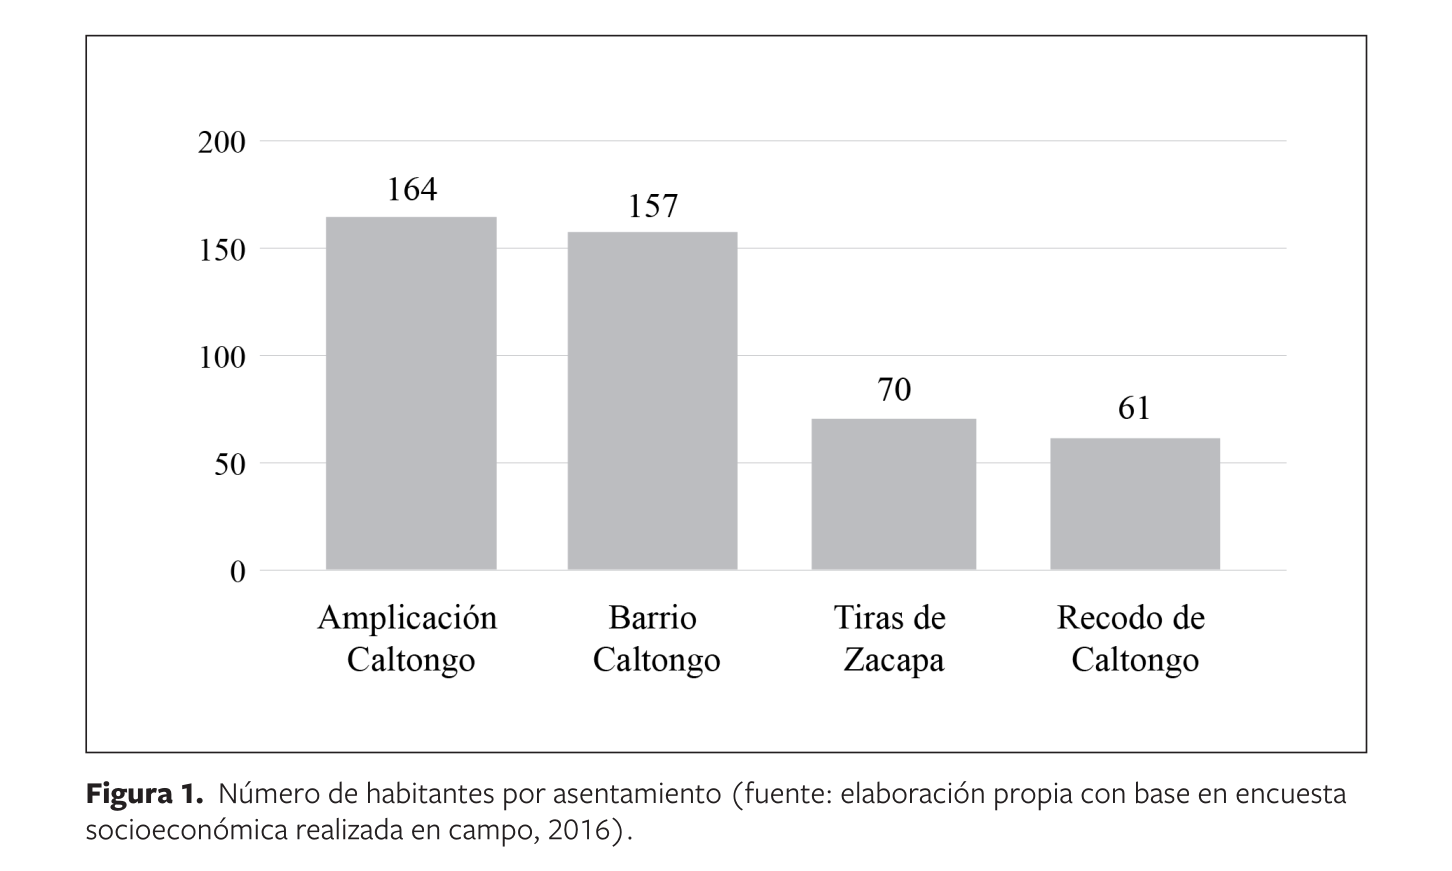
\includegraphics[width=\textwidth]{../Ensayo_Humedales/img/Fig1_Numero_habtiantes_asentamientos.png}
      \fuentefigura{Rojas Villalmar\cite{rojas2020deterioro}}
    \end{column}
    \begin{column}{0.42\textwidth}
      \begin{itemize}
        \item La ocupación irregular conlleva consecuencias ecológicas directas: al carecer de red de drenaje
        \item En Xochimilco, se estima que existen más de 1,300 descargas de aguas residuales (grises y negras) 
              vertidas directamente a los canales \cite{rojas2020deterioro}.
      \end{itemize}
    \end{column}
  \end{columns}
\end{frame}


% ── Frame con figura 2 ─────────────────────────────────────────────
\begin{frame}{Resultados del Análisis Espacial Figura 2}
  \begin{columns}[T]
    \begin{column}{0.55\textwidth}
      % Descomenta cuando tengas la imagen:
      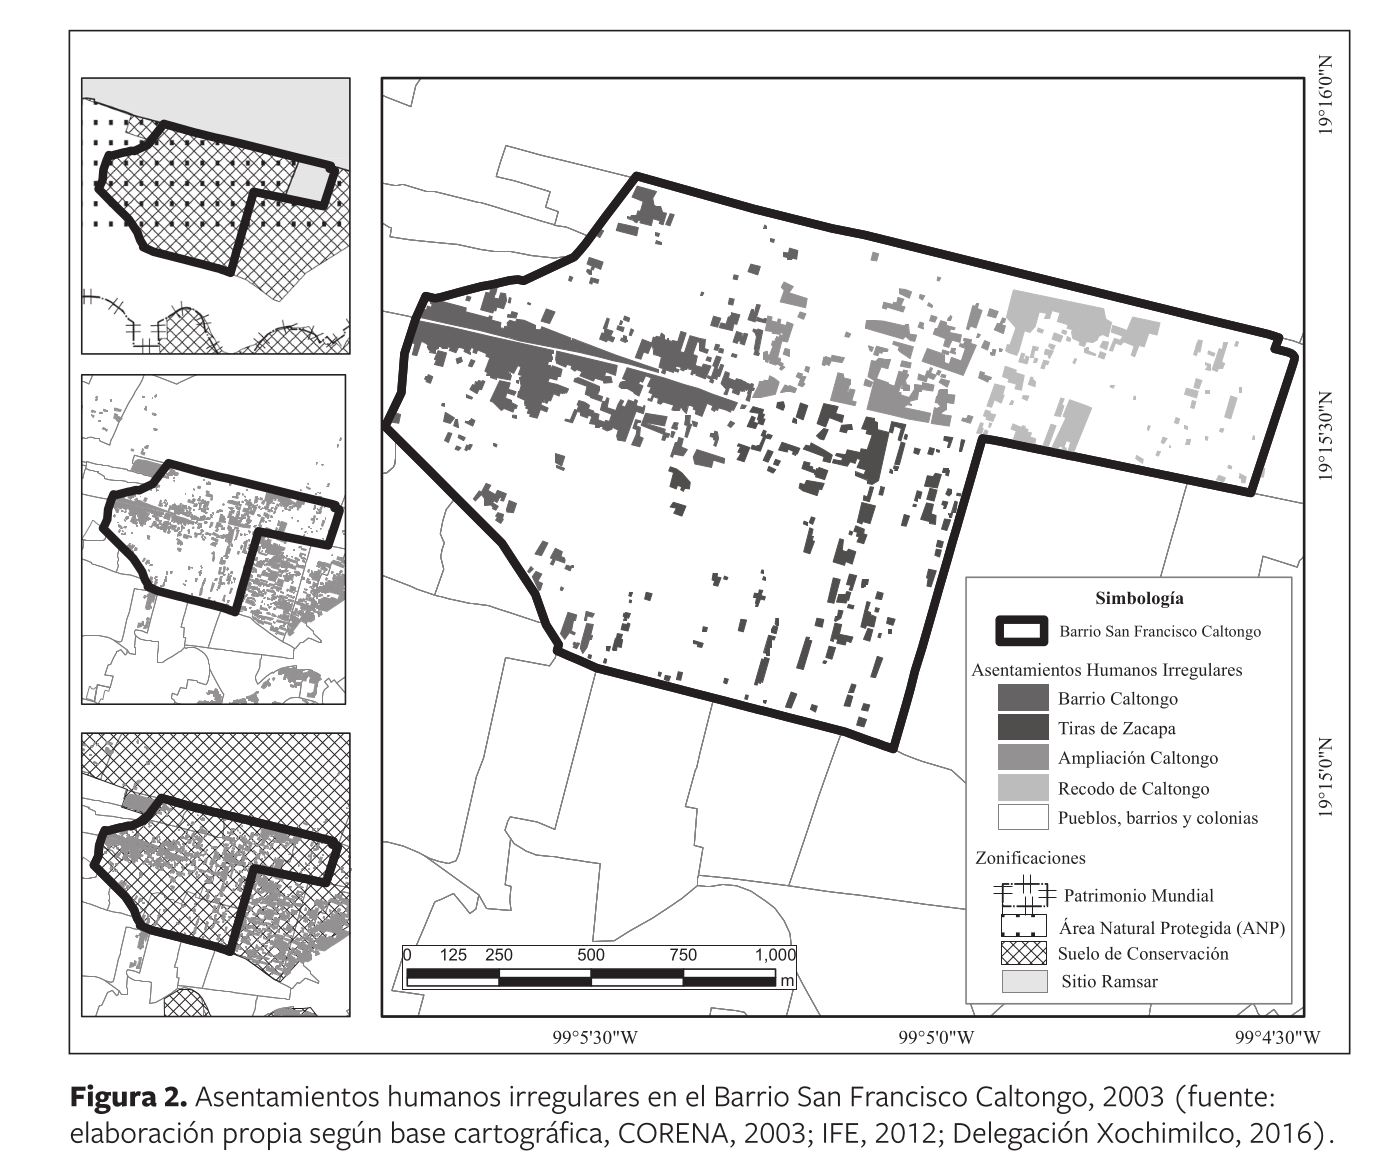
\includegraphics[width=\textwidth]{../Ensayo_Humedales/img/Fig2_Asentamientos_Humanos_irregulares.png}
      \fuentefigura{Rojas Villalmar\cite{rojas2020deterioro}}
    \end{column}
    \begin{column}{0.42\textwidth}
      \begin{itemize}
        \item Número de habitantes por asentamiento irregular en la zona lacustre.
      \end{itemize}
    \end{column}
  \end{columns}
\end{frame}

% ── Frame con figura 2 ─────────────────────────────────────────────
\begin{frame}{Resultados del Análisis Espacial Figura 3}
  \begin{columns}[T]
    \begin{column}{0.55\textwidth}
      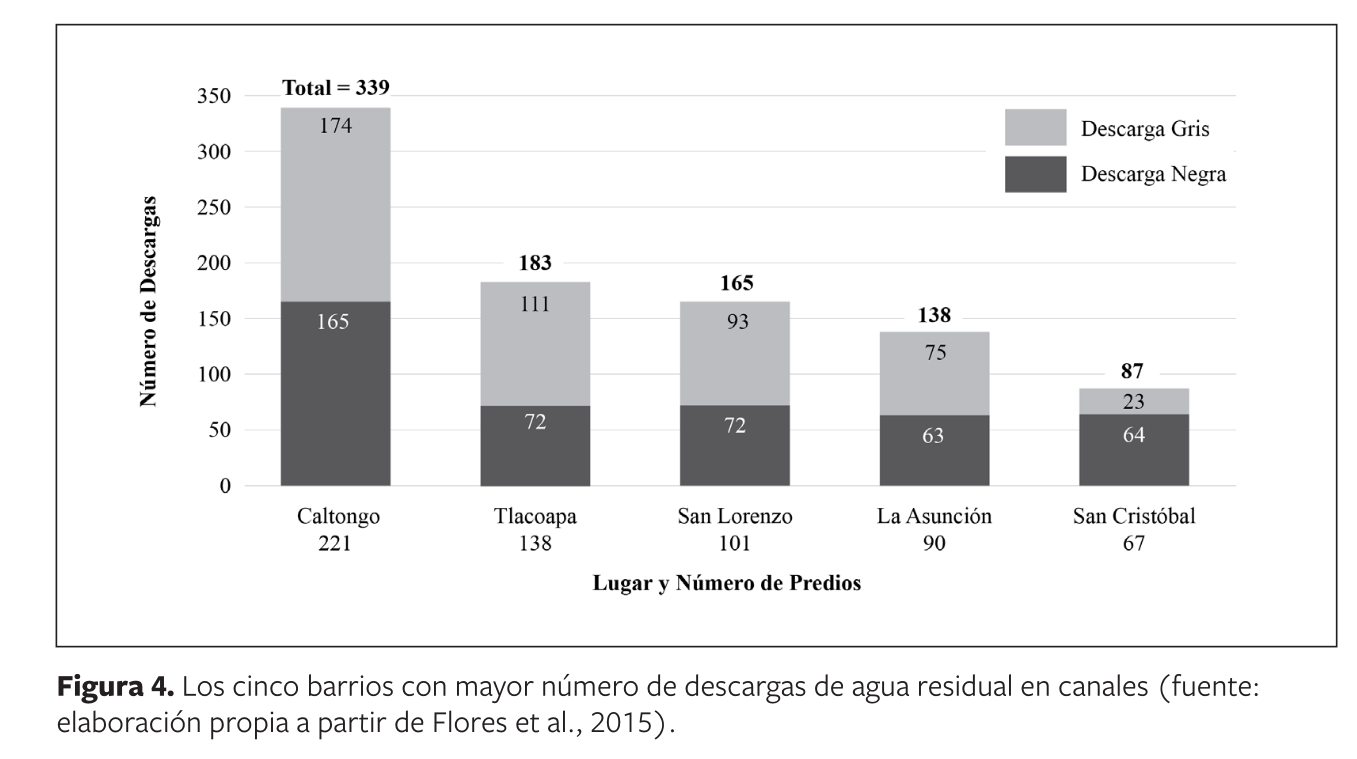
\includegraphics[width=\textwidth]{../Ensayo_Humedales/img/Fig4_Barrios_descarga.png}
      \fuentefigura{Rojas Villalmar\cite{rojas2020deterioro}}
    \end{column}
    \begin{column}{0.42\textwidth}
      \begin{itemize}
        \item Barrios con mayor número de descargas de agua residual en los canales de Xochimilco.
      \end{itemize}
    \end{column}
  \end{columns}
\end{frame}

% ── Frame: Contexto ───────────────────────────────────────────────────────────
\begin{frame}{Sustentabilidad a Largo plazo}
  \begin{itemize}
    \item \textbf{El riesgo de pérdida en Xochimilco:} El sistema lacustre de Xochimilco enfrenta un riesgo crítico de pérdida de funcionalidad 
    debido a la fragmentación del territorio. El deterioro ambiental se ha agudizado por la ausencia de red de drenaje y la proliferación de 
    descargas de aguas grises y negras directamente a los canales \cite{rojas2020deterioro}.
    \item \textbf{Impacto Social y Cultural: El Escenario de Cuemanco:} El área de Cuemanco funciona como un nodo cultural donde la identidad
 histórica se preserva mediante eventos masivos que atraen el turismo nacional e internacional, como el espectáculo de "La Llorona". 
  \end{itemize}
\end{frame}

% ── Frame: Evidencia Fotográfica (Corregido para Beamer) ────────────────────────
\begin{frame}{Evidencia Fotográfica: El Humedal de Cuemanco}
  \centering
  \begin{columns}[onlytextwidth, T] % [onlytextwidth] asegura que no se pase de los márgenes
    
    \begin{column}{0.31\textwidth}
      \centering
      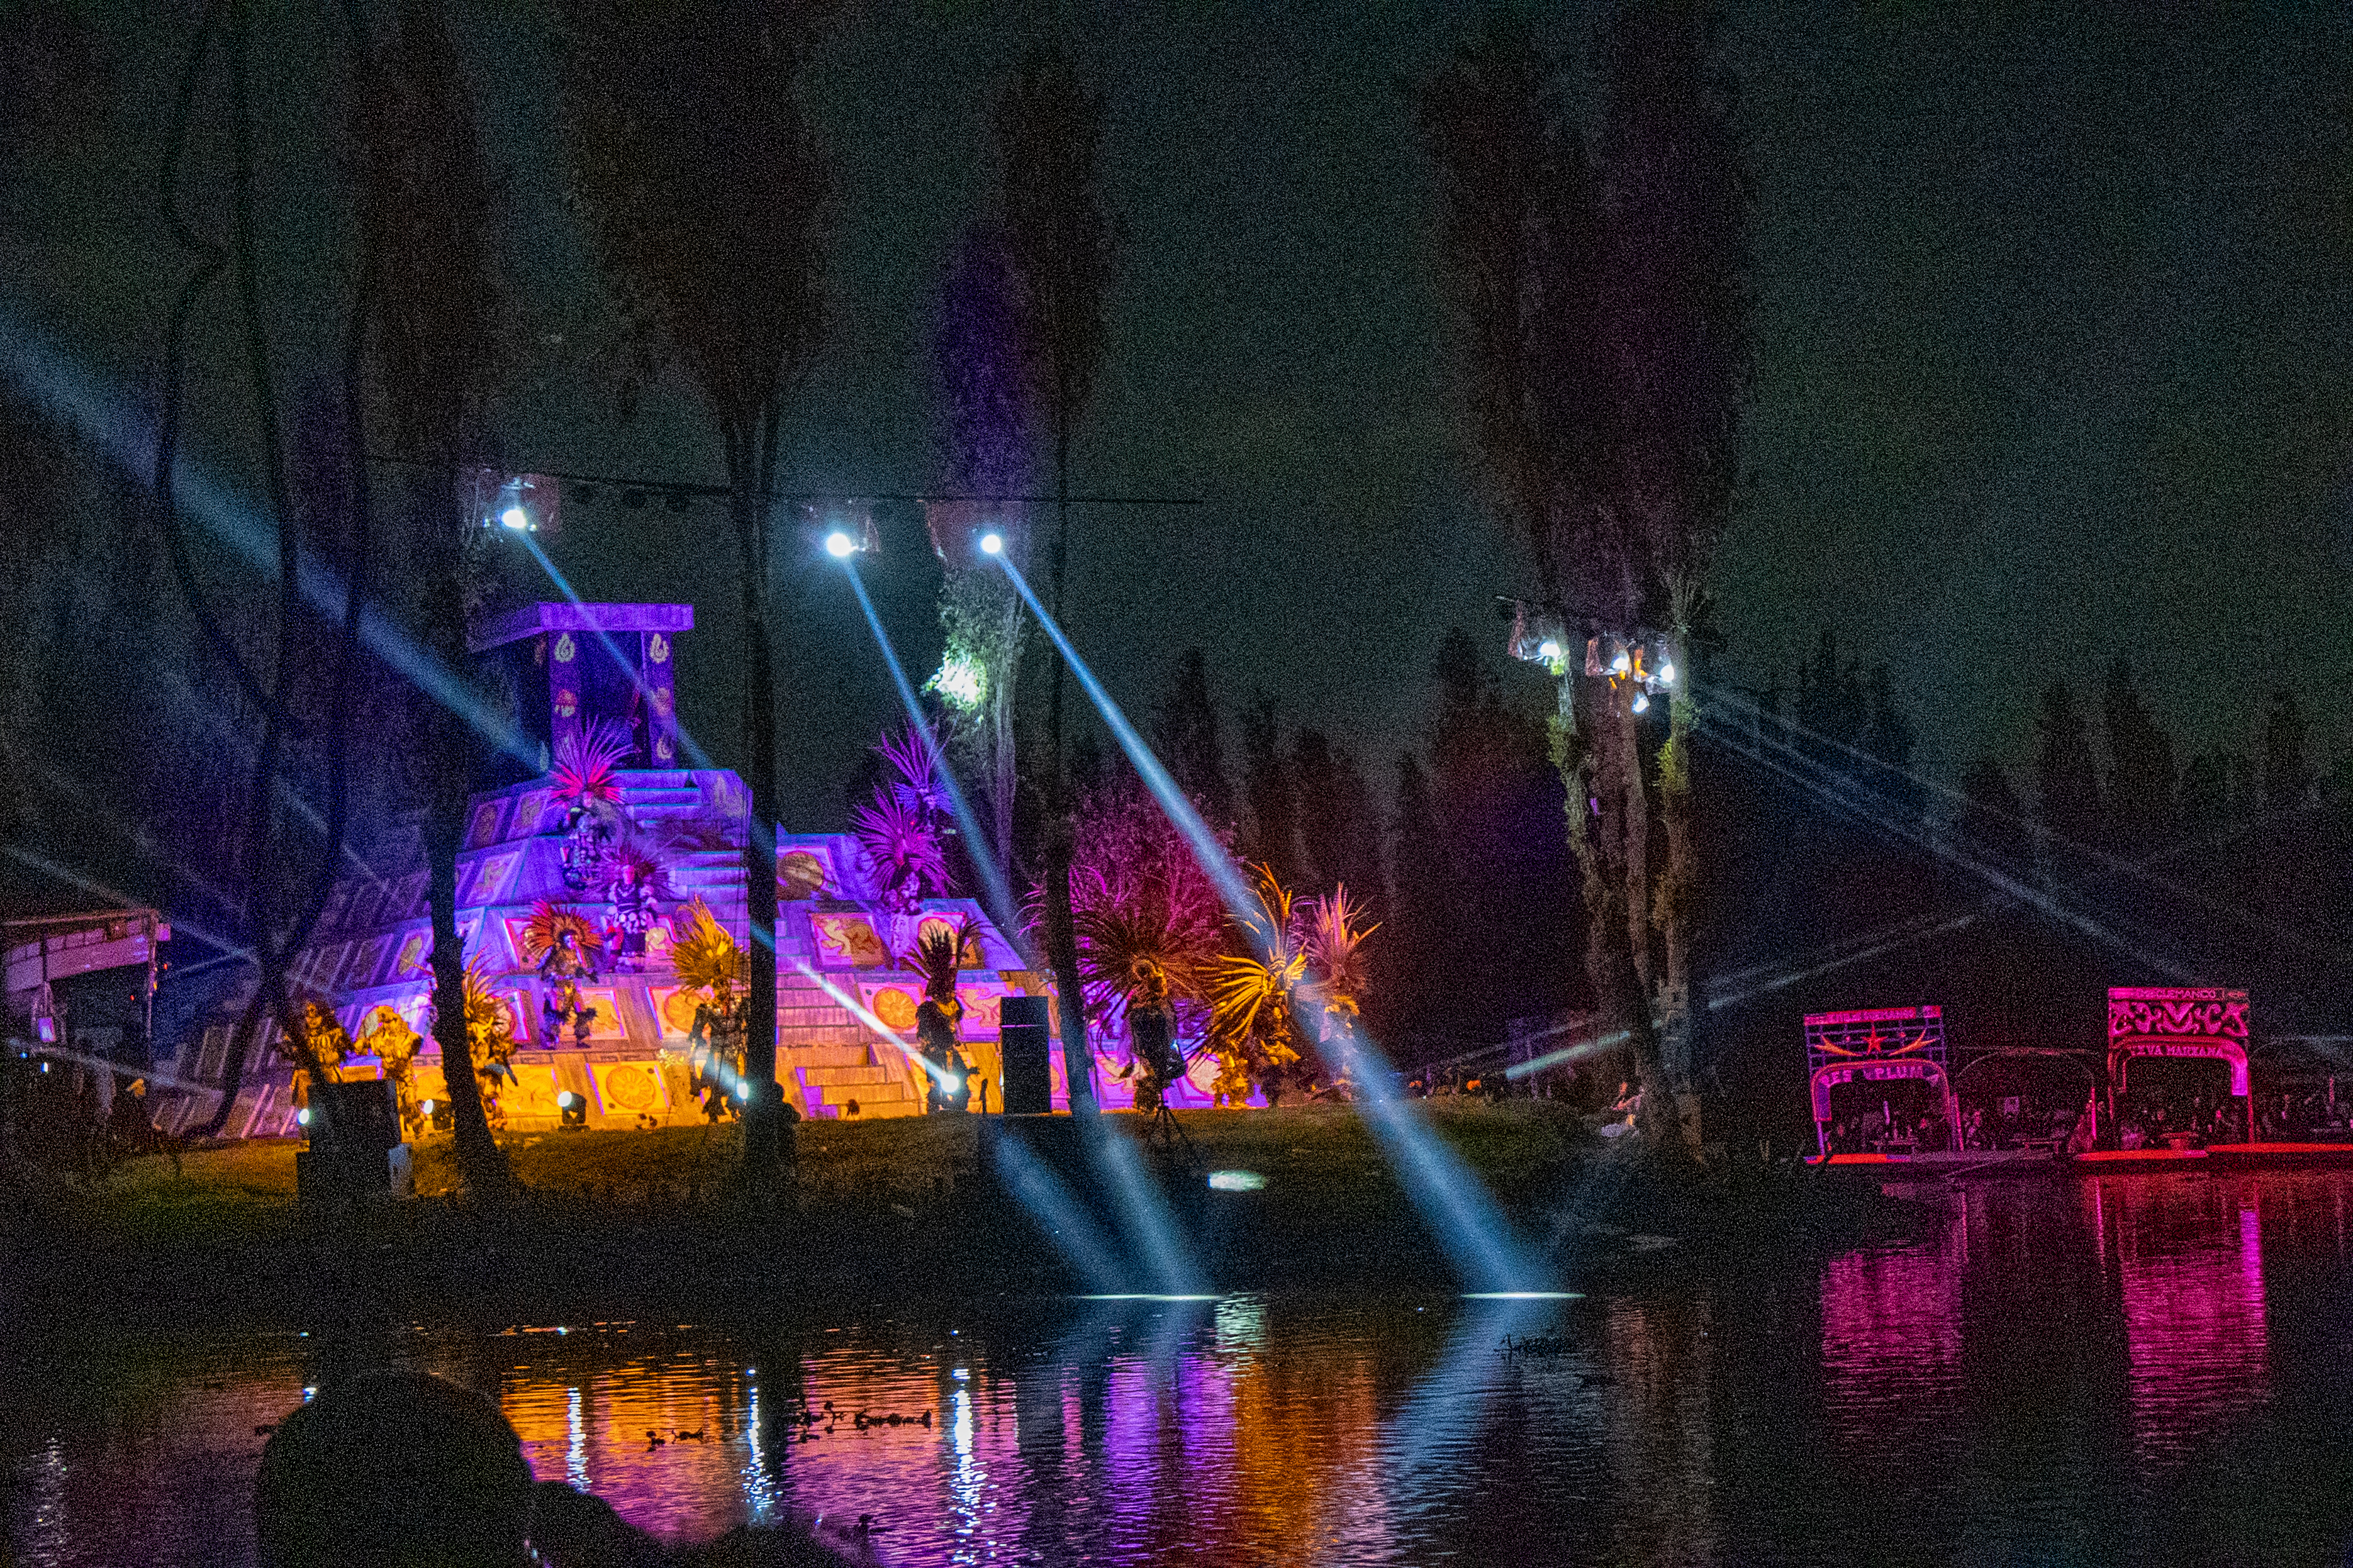
\includegraphics[width=\textwidth, height=0.4\textheight, keepaspectratio]{../Ensayo_Humedales/img/FotoLlorona3.JPEG}
      \par\scriptsize (a) Vista del escenario.
    \end{column}
    
    \hfill
    
    \begin{column}{0.31\textwidth}
      \centering
      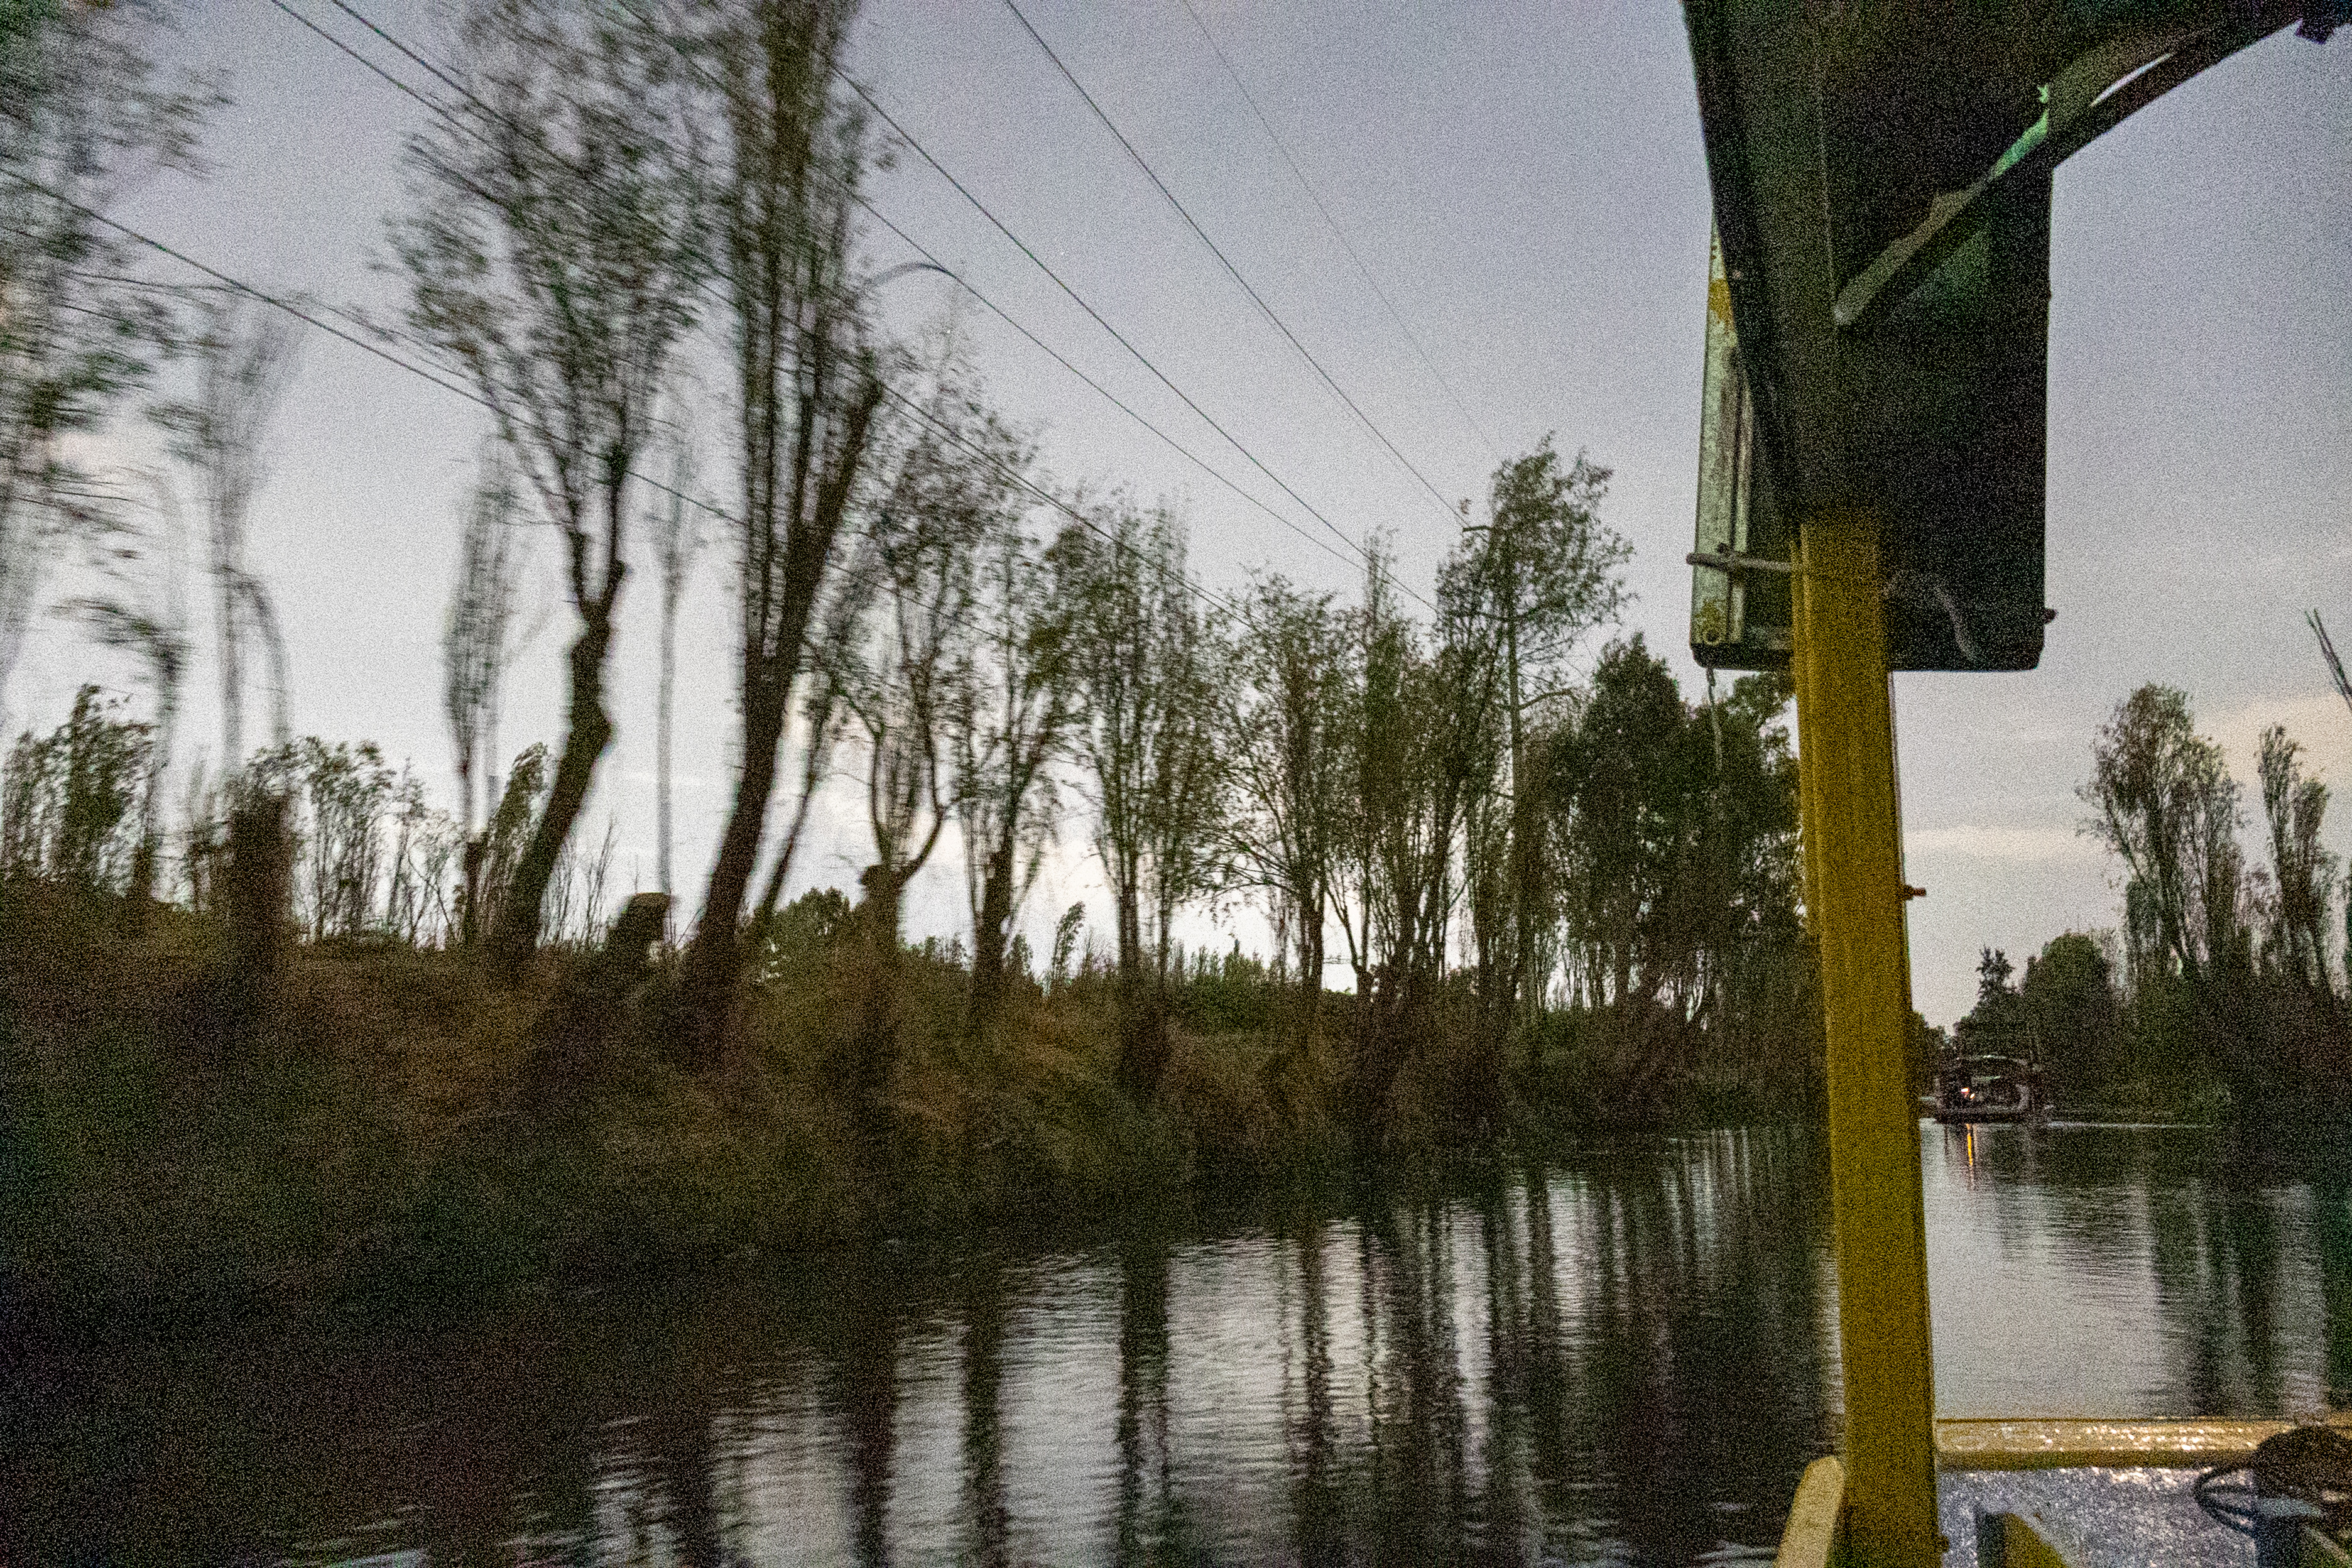
\includegraphics[width=\textwidth, height=0.4\textheight, keepaspectratio]{../Ensayo_Humedales/img/FotoLlorona2.JPEG}
      \par\scriptsize (b) Trajineras en Cuemanco.
    \end{column}
    
    \hfill
    
    \begin{column}{0.31\textwidth}
      \centering
      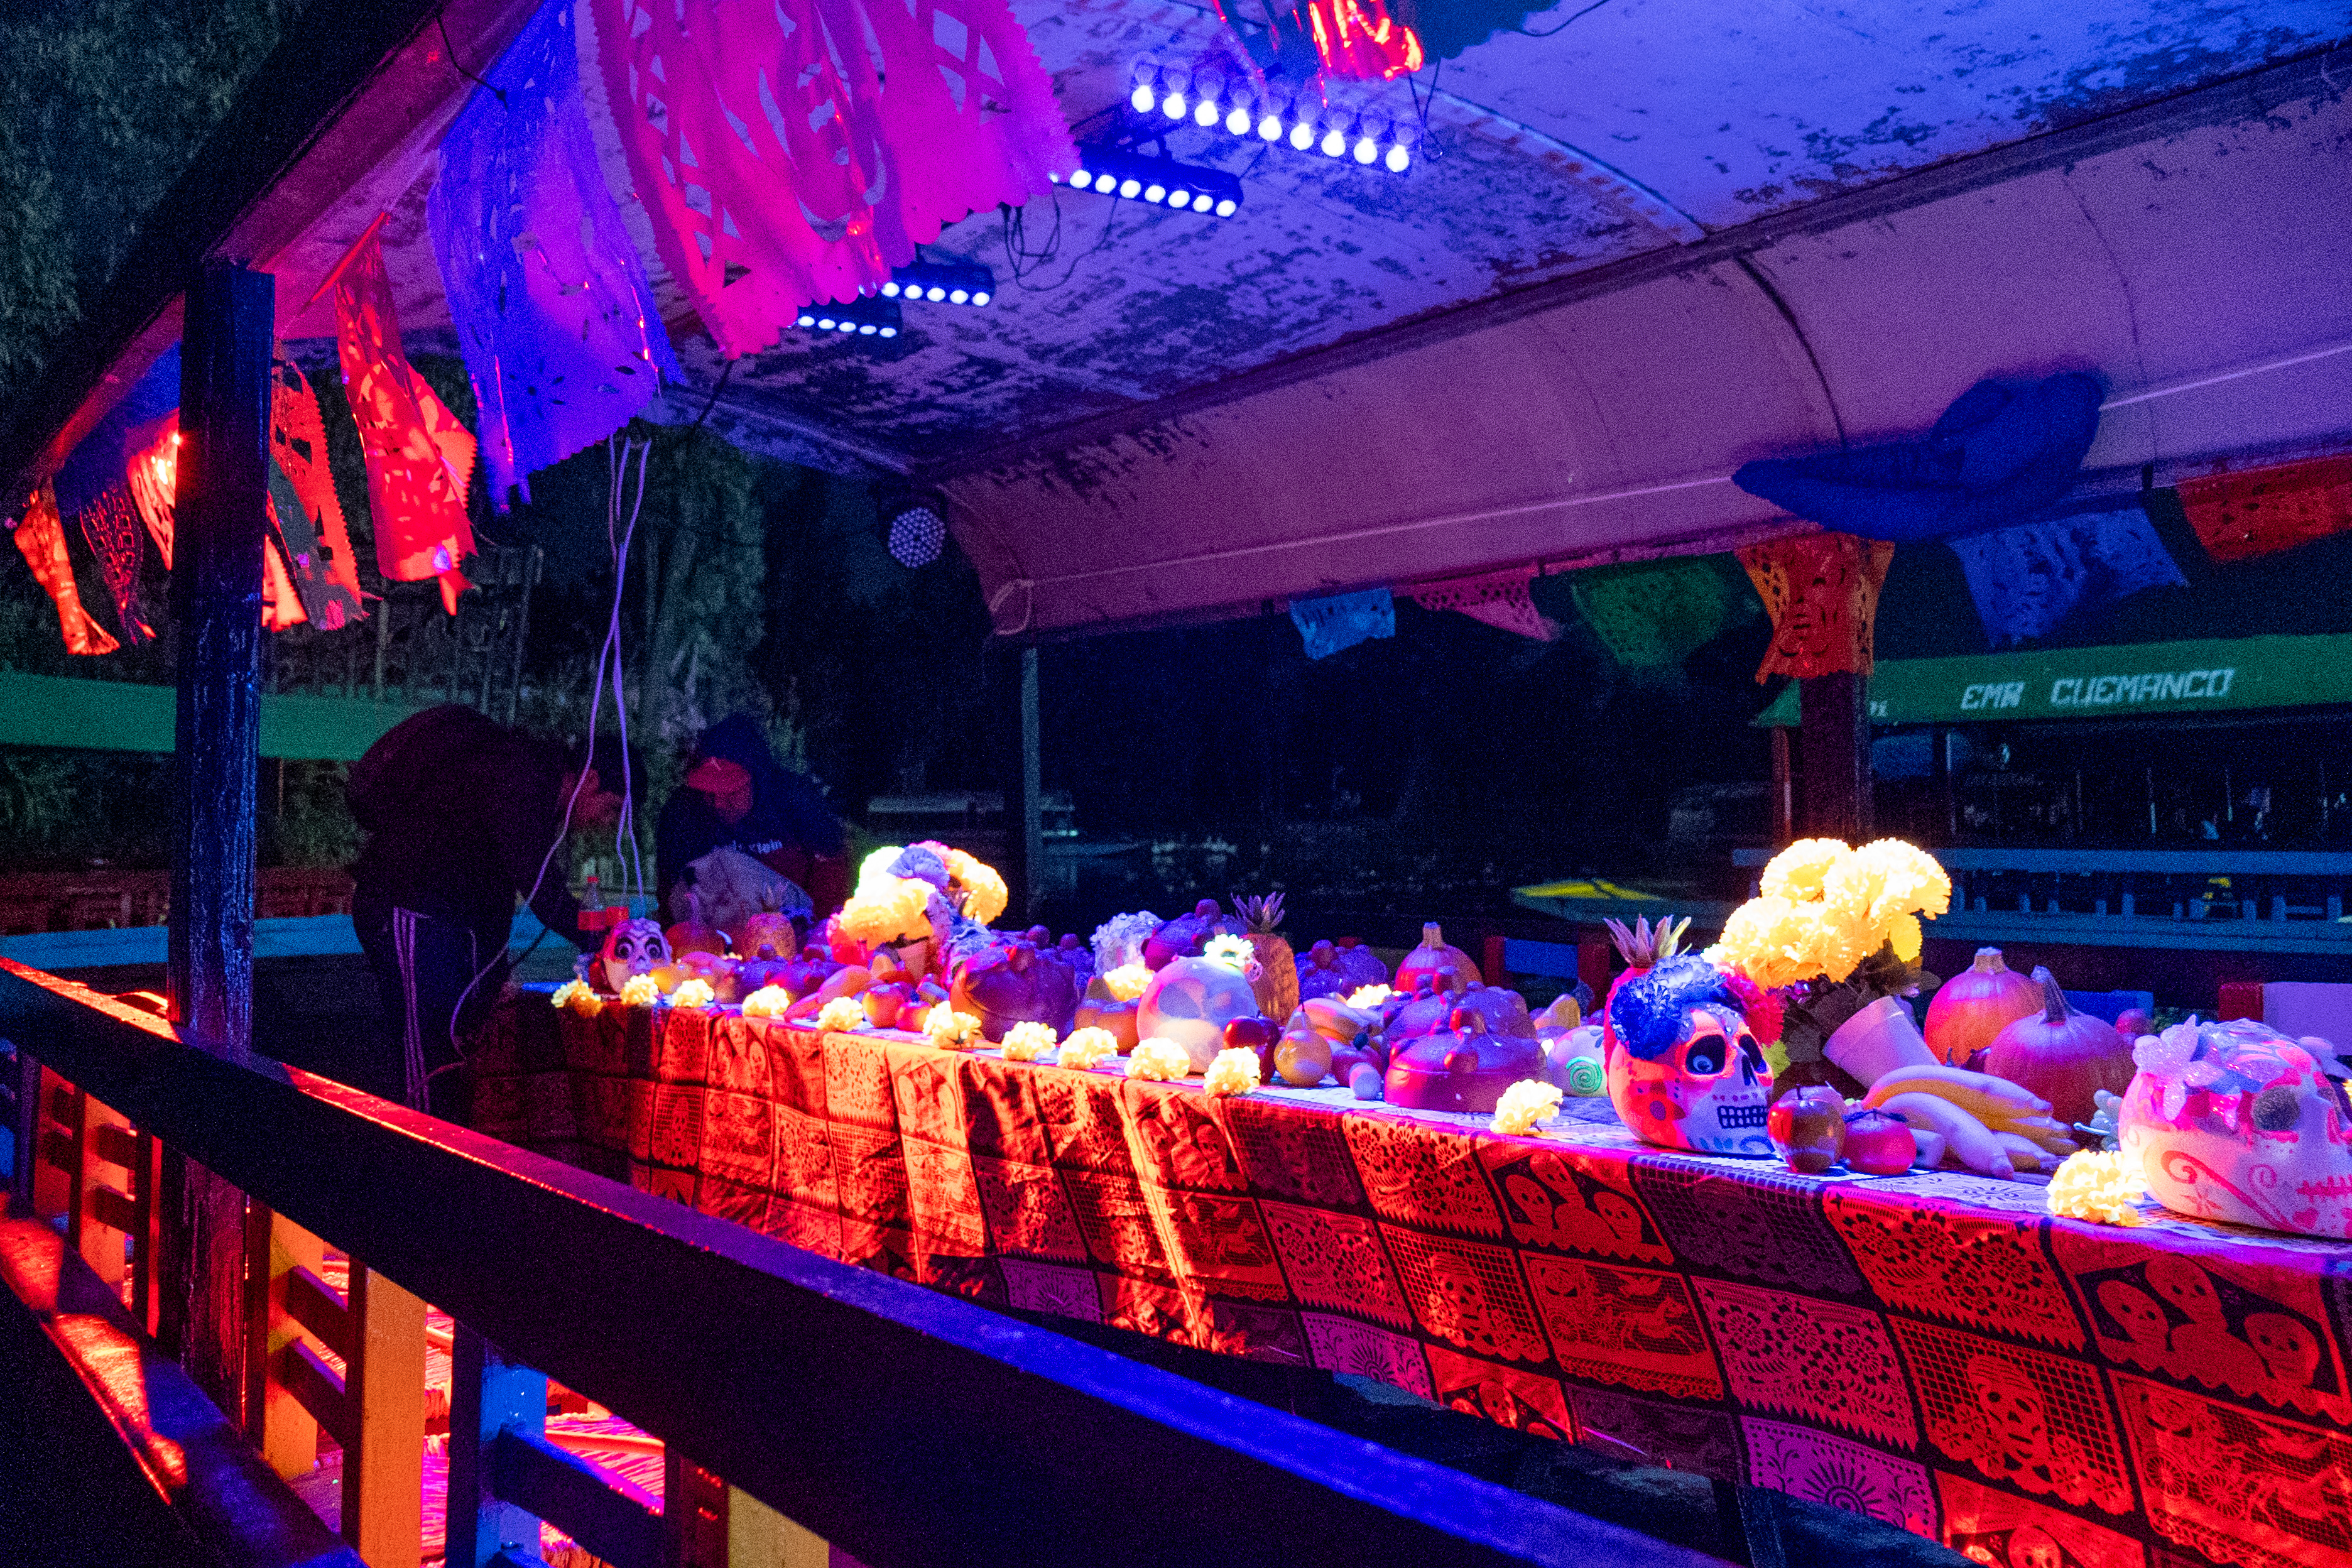
\includegraphics[width=\textwidth, height=0.4\textheight, keepaspectratio]{../Ensayo_Humedales/img/FotoLlorona1.JPEG}
      \par\scriptsize (c) Iluminación nocturna.
    \end{column}
    
  \end{columns}

  \vspace{0.5cm}
  
  {\small \textbf{Figura 4:} Espectáculo cultural en el humedal de Cuemanco.} \\
  \fuentefigura{Autoría propia, 2025.}
\end{frame}

% ── Frame: Solo texto — mensaje clave, cita o puente entre secciones ─────────
\begin{frame}[plain]
  \begin{tikzpicture}[remember picture, overlay]
    % Banda lateral de color
    \fill[ColorPrincipal]
      (current page.north west) rectangle
      ([xshift=0.35cm] current page.south west);
    % Línea dorada en el borde de la banda
    \fill[ColorAcento]
      ([xshift=0.32cm] current page.north west) rectangle
      ([xshift=0.35cm] current page.south west);
  \end{tikzpicture}
  \hspace{0.8cm}%
  \begin{minipage}{0.88\textwidth}
    \vspace{2.2cm}
    {\color{ColorAcento}\rule{0.5\textwidth}{1.2pt}}\\[0.5cm]
    {\large\bfseries\color{ColorPrincipal}
      La ingeniería ecológica en Aragón}\\[0.6cm]
    {\normalsize\color{black}
      A diferencia de la degradación por ocupación irregular, el \textbf{Bosque de San Juan de Aragón} representa un modelo 
      de remediación activa mediante la ingeniería ecológica. El objetivo principal ha sido mejorar la calidad del agua del 
      lago y recuperar la biodiversidad en una zona altamente urbanizada \cite{sedema2022programa}. El proyecto contempla la 
      intervención de 57.27 hectáreas y la operación de dos humedales artificiales; el segundo de ellos cuenta con una 
      extensión de 3,100 $m^2$ y una capacidad de filtración de 140,000 $m^3$ en 24 horas \cite{sedema2022programa}.
    }\\[0.5cm]
    {\color{ColorAcento}\rule{0.3\textwidth}{0.8pt}}
    \vfill
  \end{minipage}
\end{frame}
% ── Frame con figura 2 ─────────────────────────────────────────────
\begin{frame}{Resultados del Análisis Espacial Figura 3}
  \begin{columns}[T]
    \begin{column}{0.55\textwidth}
      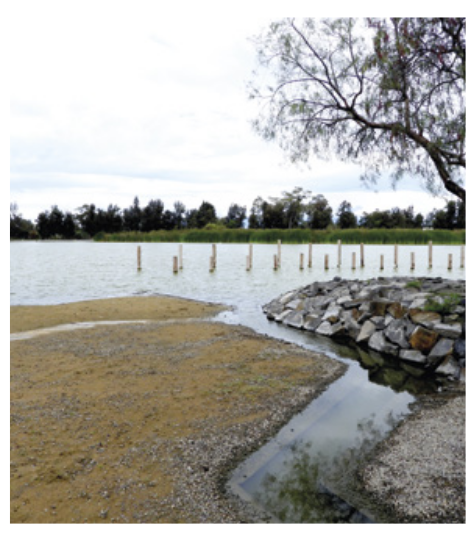
\includegraphics[width=\textwidth]{../Ensayo_Humedales/img/Aragon_vista.png}
      \fuentefigura{Vista panorámica del Bosque de San Juan de Aragón y su sistema de humedales artificiales \cite{sedema2022programa}.}
    \end{column}
    \begin{column}{0.42\textwidth}
      \begin{itemize}
        \item Esta visión de sustentabilidad destaca por la participación de la comunidad universitaria.
        \item Un equipo interdisciplinario de la UNAM ha desarrollado tecnología propia para estos 
              sistemas de tratamiento biológico, demostrando que la academia puede generar soluciones basadas en la naturaleza.
      \end{itemize}
    \end{column}
  \end{columns}
\end{frame}